\section{商品评论标签爬取}

苏宁的域名组织较有规律,这也是我们选它作为目标网站的原因之一。对于商品详情页,其组织形式是“https://product.suning.com/\{\}/\{\}.html.format(shop, sku)”,其中shop是10位的一串商铺代号,如苏宁自营是“0000000000”。后面的sku是11位的商品代号,如Apple Watch是“11357287387”。整体来说,实现苏宁商品评价的思路和京东的类似,主要差别就在于上面的参数由京东的一个商品productID变为了苏宁的商铺ID和商品ID。那么将爬虫的处理商品评价的函数改为双参数即可。
\begin{python}
def crawl_sn_cmt_tag(sku, shop):# change for url
\end{python}

然而还有一个不同是,苏宁的评价内容,标签,以及统计信息放在三个不一样的url。我们通过上面京东部分介绍过的寻找请求url的方法可以分别找到对应的目标url。

我们找到了tags的位置\ref{yhb111}:
(篇幅所限,略去过程)
\begin{figure}[htbp]
\centering
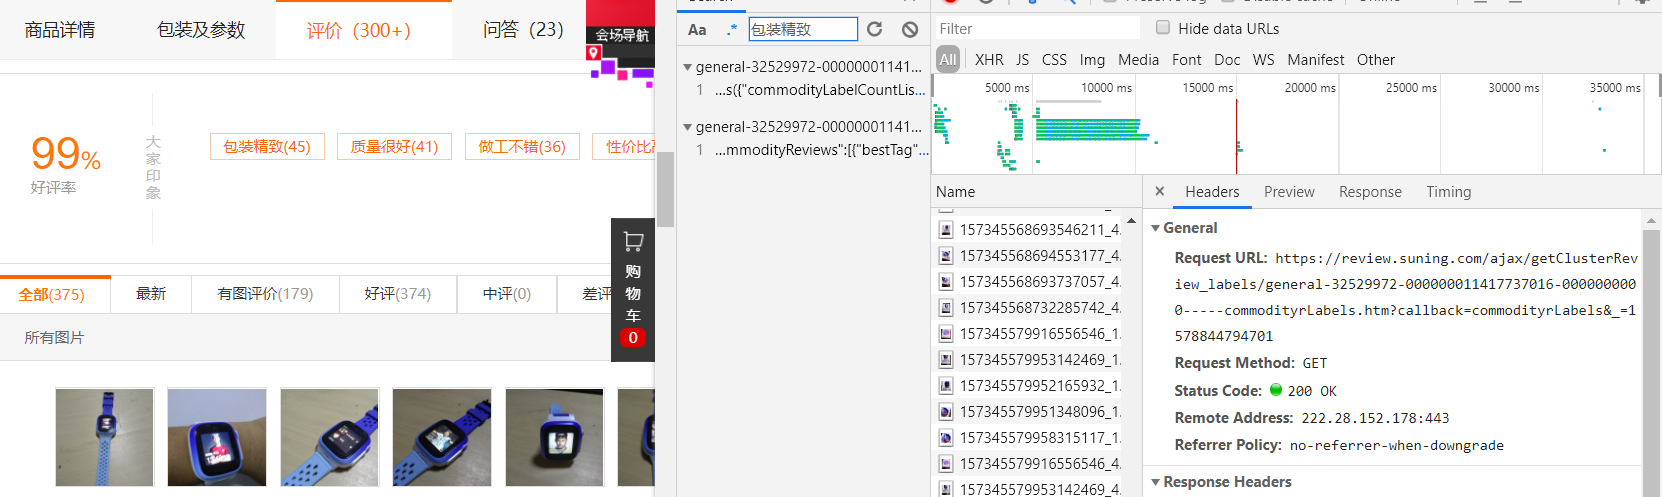
\includegraphics[width=13.5cm]{img/yhb/sn_eg2.png}
\caption{在文件夹中显示}
\label{img:yhb111}   % 引用标记,用于文章中引用
\end{figure}

抽取商铺和商品ID得到:
\begin{python}
url=r"https://review.suning.com/ajax/" \
        r"getClusterReview_labels/cluster-33667504-0000000" \
        r"{}-{}" \
        r"-----commodityrLabels.htm?".format(sku,shop)
\end{python}


先不说找这个url是一个很费工的事情,我们在如何处理“32762695“这串数字上纠结了一段时间——它并不代表商品的某种属性。后来想得更直接了一点:”既然没有关系,就把它当作都可以用的吧“,像对待京东商品ID前面那一串一样处理即可。事实证明,这种做法是有效的。

在调用json库转换对象之后,面临的问题就和之前在京东解决过的一模一样了。对京东标签的代码稍加修改即可。此外,需要注意有的商品ID不足11位,需要进行补足:
\begin{python}
while (len(sku) < 11):
                sku = "0" + sku
\end{python}


爬取结果示例如下\ref{img:yhb100}:
\begin{figure}[htbp]
\centering
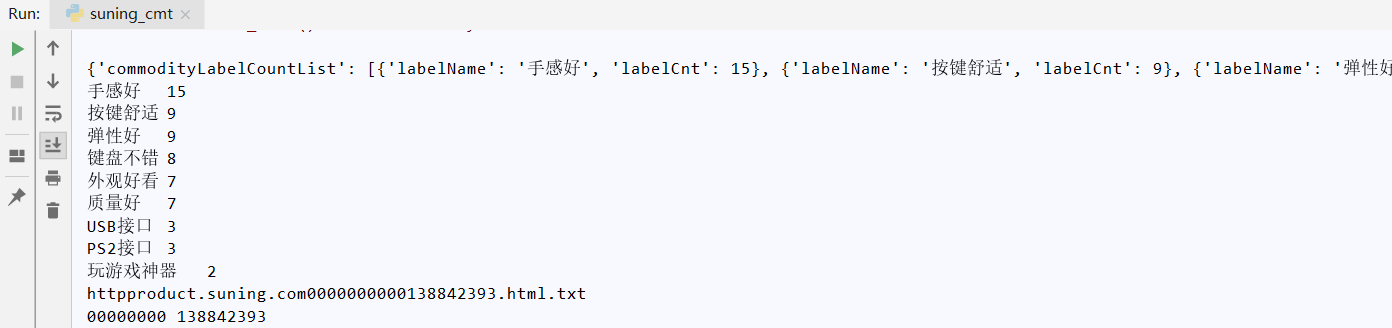
\includegraphics[width=13.5cm]{img/yhb/sn_res1.png}
\caption{在文件夹中显示}
\label{img:yhb100}   % 引用标记,用于文章中引用
\end{figure}

\section{商品评分计算}

根据前述方法,统计信息的位置在\ref{img:yhb121}:
\begin{figure}[htbp]
\centering
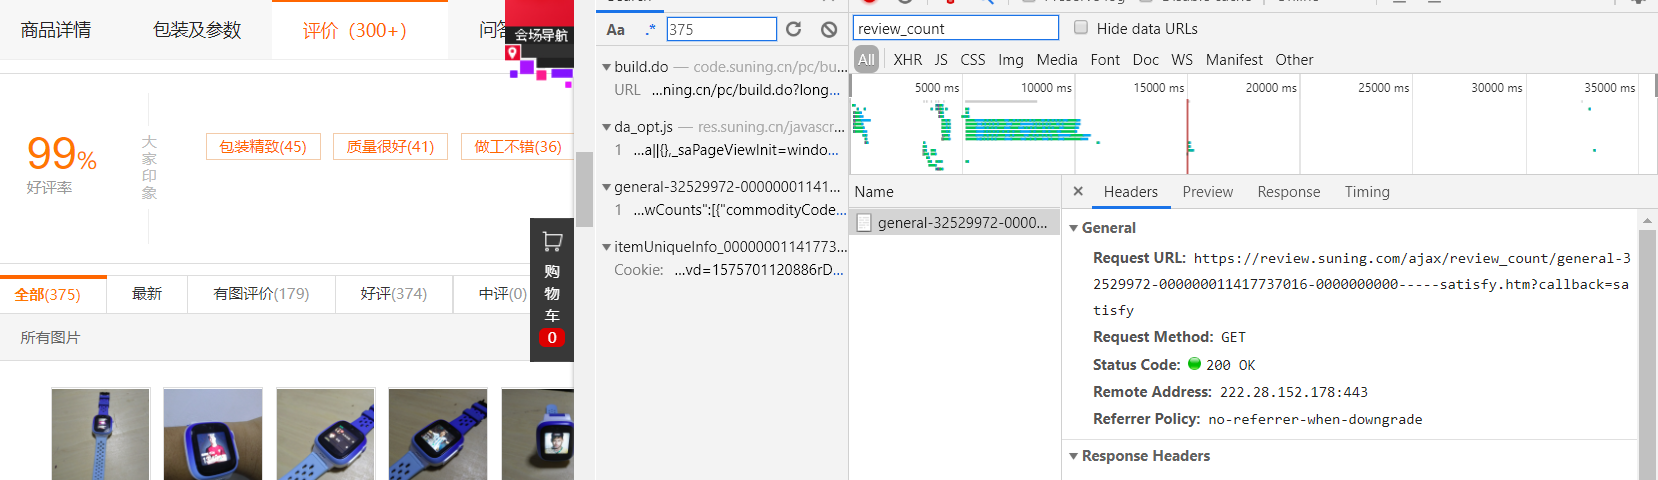
\includegraphics[width=13.5cm]{img/yhb/sn_eg.png}
\caption{在文件夹中显示}
\label{img:yhb121}   % 引用标记,用于文章中引用
\end{figure}

抽取商铺和商品ID得到:
\begin{python}
url=r"https://review.suning.com/ajax/" \
        r"review_count/cluster-32762695-0000000" \
        r"{}-{}" \
        r"-----satisfy.htm?".format(sku,shop)
\end{python}
评分结果示例如下\ref{img:yhb101}:
\begin{figure}[htbp]
\centering
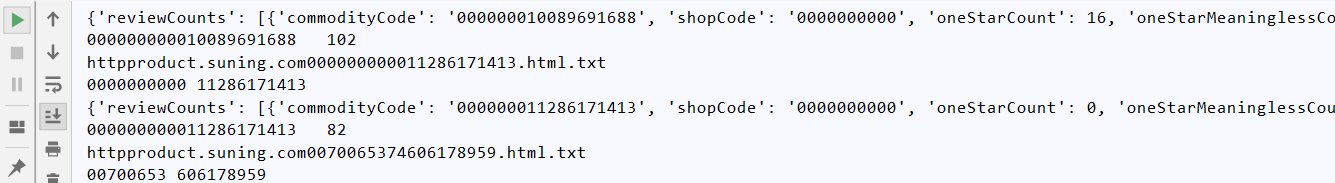
\includegraphics[width=13.5cm]{img/yhb/sn_res2.png}
\caption{在文件夹中显示}
\label{img:yhb101}   % 引用标记,用于文章中引用
\end{figure}


%%%%%%%%%%%%%%%%%%%%%%
以上就是京东和苏宁爬虫的全部内容了,到这里主要完成了信息准备和预处理的工作。
下面,我们将介绍索引(包括图片)的构建和搜索功能的实现过程。




